
\subsection{Hierarchical Aerodynamic Knowledge Learning}
\label{sec:knowledge-learning}

The source-domain aerodynamic knowledge is represented at two complementary levels: the baseline sectional pressure response and the regional pressure corrections associated with finite-span effects. The sectional model provides baseline pressure distributions and reusable aerodynamic features, while the regional models learn root and tip pressure corrections conditioned on the sectional response. Their transfer and spatial combination on the target wing are described in Sec.~\ref{sec:knowledge-projection}.

\subsubsection{Sectional Baseline Pressure Model}
\label{sec:sectional-baseline}

The sectional baseline model predicts the pressure distributions of infinite-span swept wings from airfoil geometry and flow conditions. The upper and lower surfaces are represented on separate chordwise grids, each containing three input channels: the normalized surface ordinate $y/c$, an affinely rescaled chordwise coordinate $x/c$, and the logarithm of the local nodal spacing relative to its mean. The flow-condition vector is defined as $\boldsymbol{\mu}=[M_\infty,\alpha,\Lambda,\log_{10}(Re/10^{7})]^{\mathsf T}$. The geometric ordinates and flow conditions are standardized using statistics from the training partition. The model predicts the upper- and lower-surface pressure distributions as
\begin{equation}
    \left(\widehat{\mathbf C}_{p,u}^{\mathrm{sec}},
          \widehat{\mathbf C}_{p,l}^{\mathrm{sec}}\right)
    =\mathcal F_{\mathrm{sec}}\!\left(\mathbf G_u,\mathbf G_l,\boldsymbol{\mu}\right),
    \label{eq:sectional-baseline-map}
\end{equation}
where $\mathbf G_s\in\mathbb R^{3\times N_s}$ denotes the coordinate representation of surface $s\in\{u,l\}$, and $N_s$ is the corresponding number of chordwise nodes.

The network architecture is illustrated in Fig.~\ref{fig:sectional-architecture}. It consists of two surface-specific convolutional branches, a shared flow-condition encoder, and a global feature-fusion module. The condition encoder maps the four-dimensional flow-condition vector into a 128-dimensional embedding $\mathbf h$. For each surface, an initial one-dimensional convolution maps the three input channels to 128 feature channels, followed by eight FiLM-modulated residual blocks with dilation factors $(1,2,4,1,2,4,1,2)$. The flow-condition embedding modulates the intermediate features through feature-wise linear modulation (FiLM), expressed as
\begin{equation}
    \widetilde{\mathbf H}
    =\left[\mathbf 1+\boldsymbol\gamma(\mathbf h)\right]
    \odot \operatorname{GN}(\mathbf H)+\boldsymbol\beta(\mathbf h),
    \label{eq:sectional-film}
\end{equation}
where $\operatorname{GN}$ denotes group normalization, and $\boldsymbol\gamma$ and $\boldsymbol\beta$ are condition-dependent channelwise modulation parameters. The residual blocks extract chordwise features at multiple receptive-field scales without downsampling, preserving the original nodal resolution of each surface.

To incorporate information from both surfaces, the extracted features are independently aggregated into 128-dimensional vectors through quadrature-weighted pooling. These vectors are concatenated with the condition embedding $\mathbf h$ and passed through a shared fusion network with dimensions $384\rightarrow256\rightarrow256$. The resulting global representation is divided into two 128-dimensional feature increments, which are broadcast along the corresponding chordwise grids and added to the surface-specific features. Separate prediction heads then map the fused features to the upper- and lower-surface pressure coefficients. This design preserves independent surface representations while allowing the two branches to exchange global aerodynamic information.

The sectional model is trained using the CFD pressure distributions of the infinite-span swept-wing database. The training objective is the equally weighted mean squared error of the upper- and lower-surface predictions, excluding the first chordwise node on each surface because of discontinuities in the corresponding CFD labels. After pretraining, the model provides baseline sectional pressure predictions for the regional correction models, while its intermediate features are retained for subsequent target-domain residual learning in Sec.~\ref{sec:target-residual}.

\begin{figure*}[t]
    \centering
    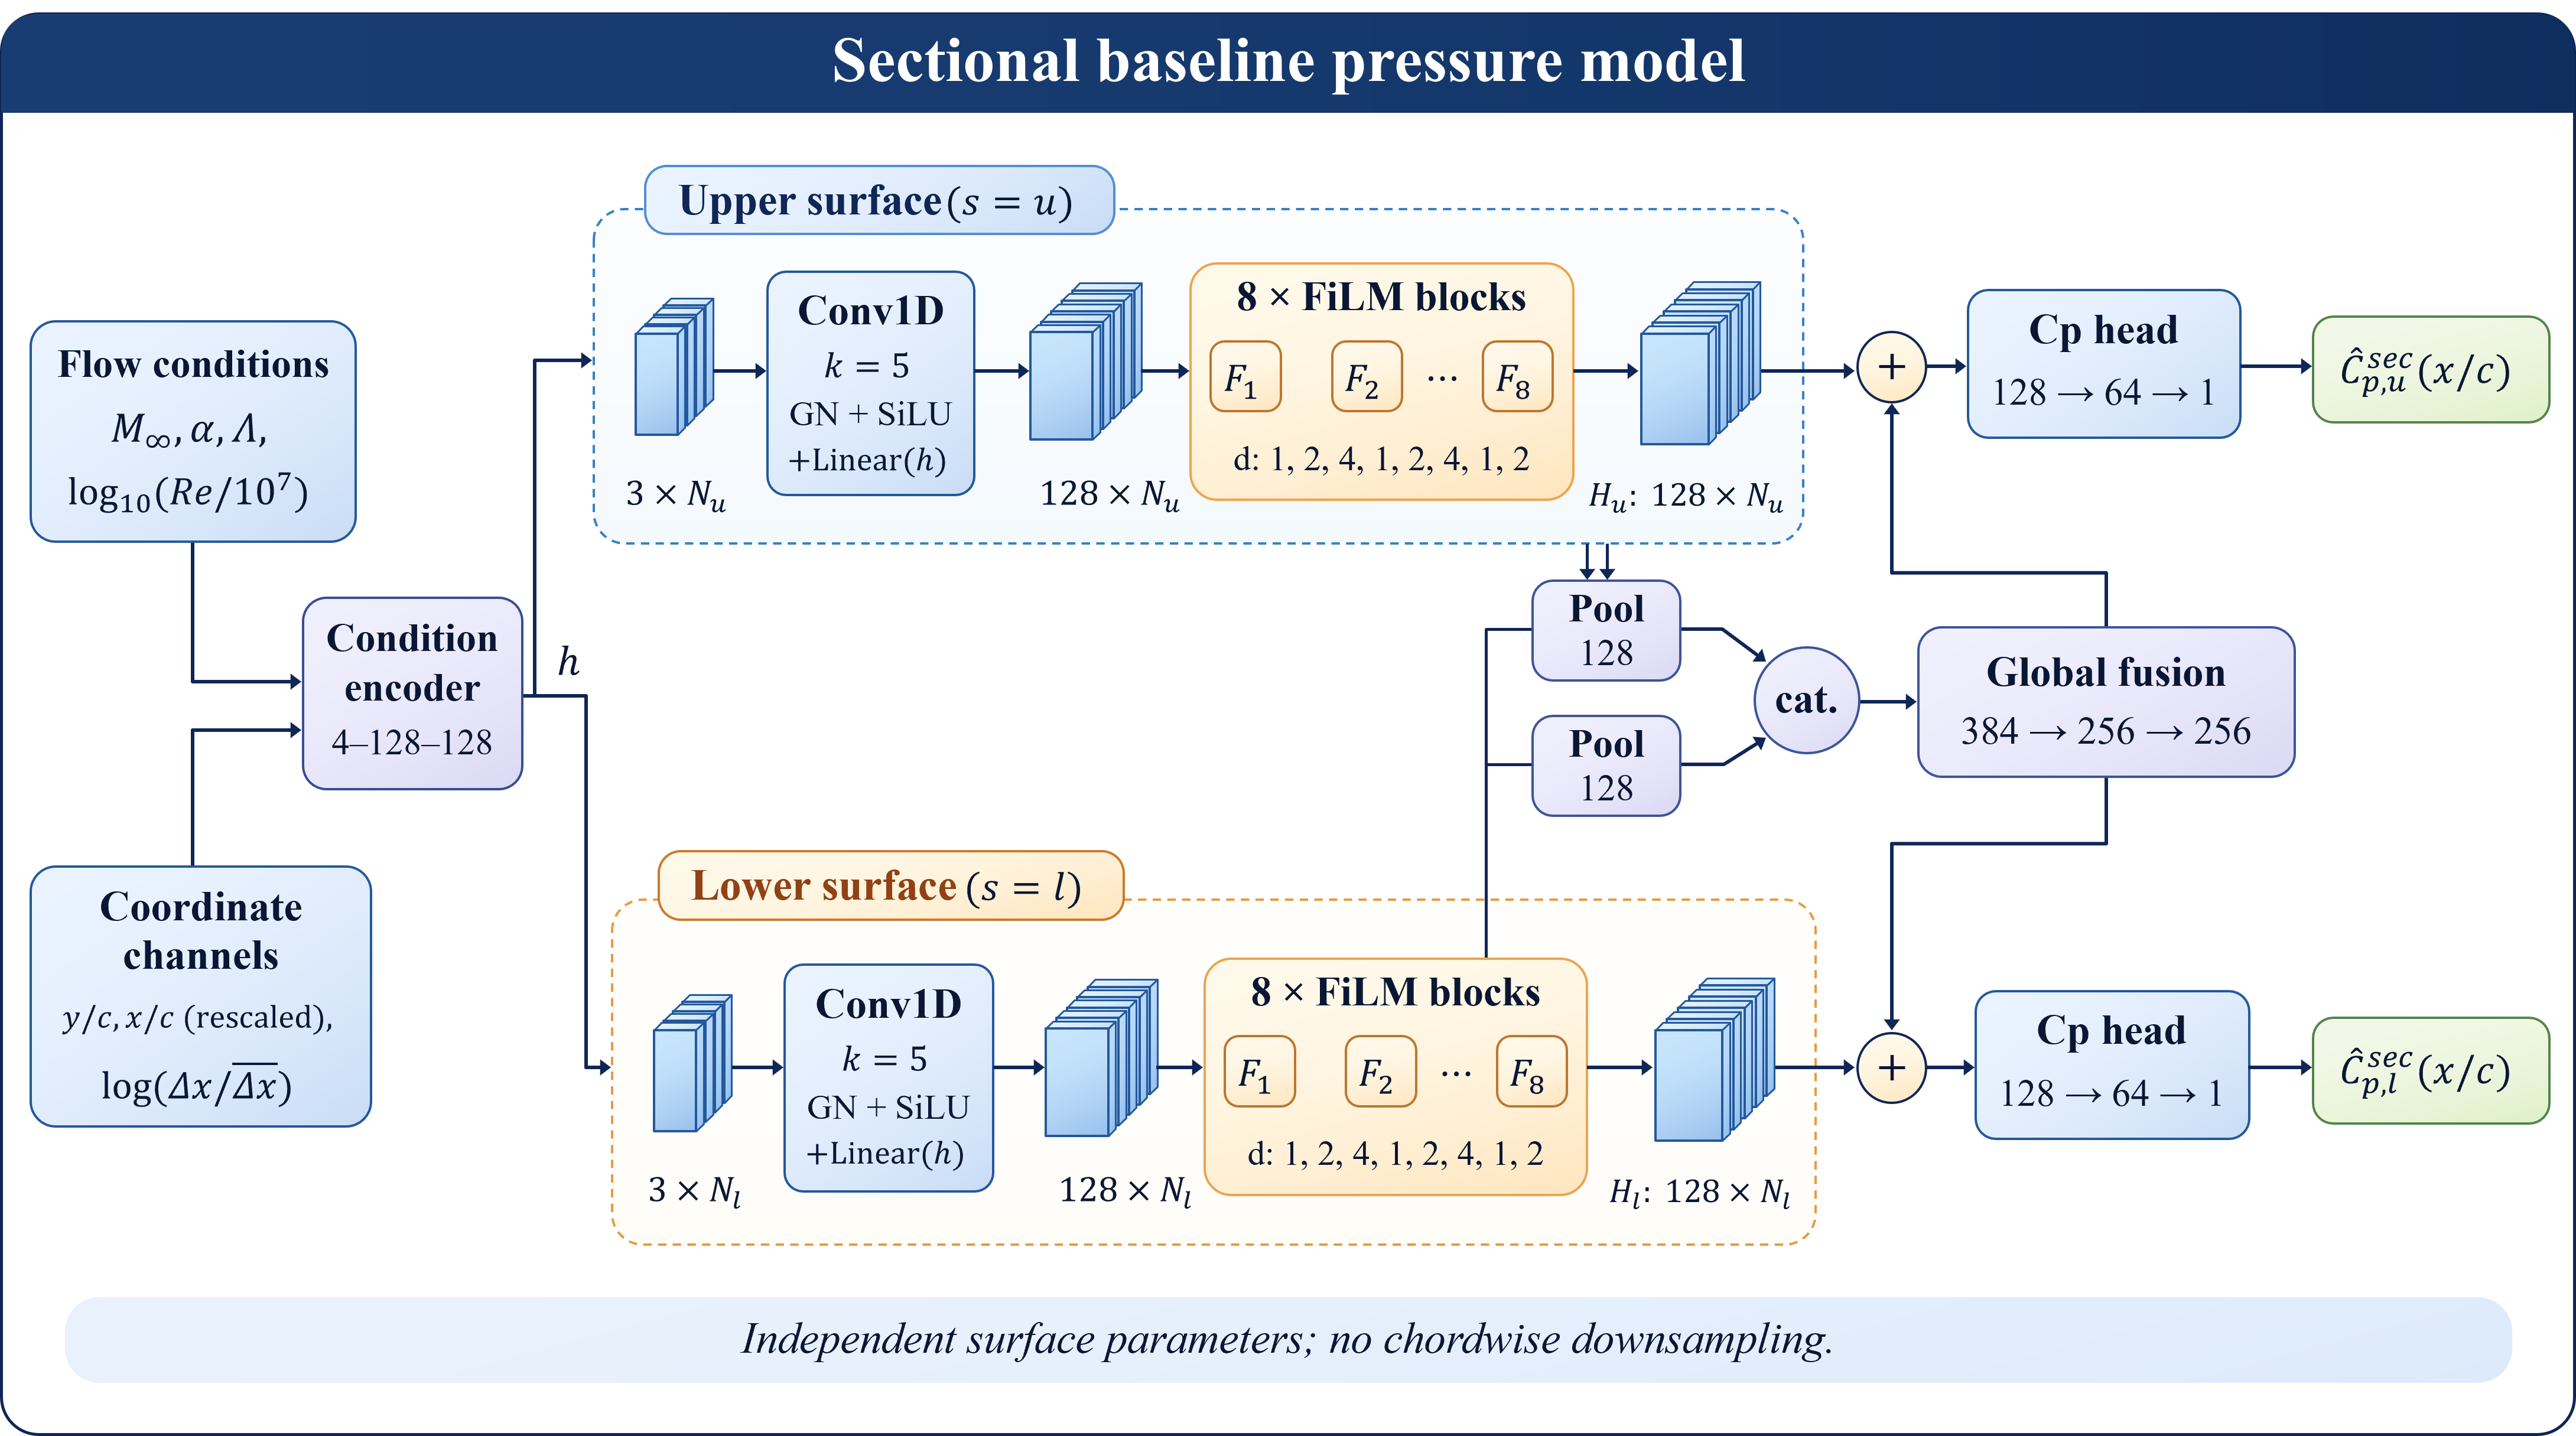
\includegraphics[width=0.98\textwidth]{III_Knowledge_Transfer/figures/III_B_Fig09/III_B_Fig09_sectional_architecture.png}
    \caption{Architecture of the sectional baseline pressure model with surface-specific convolutional branches and shared global feature fusion.}
    \label{fig:sectional-architecture}
\end{figure*}



\subsubsection{Regional Finite-Span Correction Models}
\label{sec:regional-correction}

The regional correction models are developed to capture pressure variations associated with finite-span effects near the wing root and tip that are not represented by the sectional baseline response. For geometrically and aerodynamically matched finite- and infinite-span CFD cases, the pressure discrepancy is defined as
\begin{equation}
    \Delta C_{p,s}^{\mathrm{CFD}}(d,\xi)
    = C_{p,s}^{\mathrm{fin,CFD}}(d,\xi)
    - C_{p,s}^{\infty,\mathrm{CFD}}(\xi),
    \qquad s\in\{u,l\},
    \label{eq:regional-cfd-discrepancy}
\end{equation}
where $\xi=x/c$ is the normalized chordwise coordinate and $d$ denotes the distance from the corresponding spanwise boundary. The correction targets are obtained directly from paired CFD solutions rather than from discrepancies relative to the learned sectional predictions.

For the root region, the correction model incorporates airfoil geometry, flow conditions, the normalized root-distance coordinate $d_r$, and the upper- and lower-surface pressure distributions predicted by the pretrained sectional model. The corresponding mapping is expressed as
\begin{equation}
    \left(\widehat{\Delta\mathbf C}_{p,r,u},
          \widehat{\Delta\mathbf C}_{p,r,l}\right)
    =\mathcal F_r\!\left(
    \mathbf G_u,\mathbf G_l,\boldsymbol\mu,d_r,
    \widehat{\mathbf C}_{p,u}^{\mathrm{sec}},
    \widehat{\mathbf C}_{p,l}^{\mathrm{sec}}
    \right),
    \label{eq:root-correction-map}
\end{equation}
where the sectional model remains frozen during regional training. Its predicted pressure distributions provide aerodynamic conditioning information, while the root-distance coordinate characterizes the spanwise variation in the pressure correction.

The root-region correction network is illustrated in Fig.~\ref{fig:regional-architecture}. To accommodate the different chordwise discretizations of the upper and lower surfaces, the lower-surface geometry and predicted sectional pressure are interpolated onto the upper-surface grid. The resulting input contains four surface channels, comprising the upper- and lower-surface ordinates and their corresponding sectional pressure predictions, together with five broadcast conditioning channels and one normalized chordwise-coordinate channel. These ten channels are processed by a Conv1D stem followed by six multiscale residual blocks with dilation factors $(1,2,4,2,1,2)$. A zero-initialized two-channel prediction head produces pressure corrections for both surfaces on the common grid, after which the lower-surface correction is interpolated back to its original chordwise grid. Each spanwise section is processed independently.

The multiscale residual blocks combine conventional and dilated convolutions with channel mixing and residual connections to extract pressure-discrepancy features at different chordwise scales. The correction model is trained using an unweighted pointwise mean squared error over the retained upper- and lower-surface nodes, without additional shock- or gradient-dependent weighting. An analogous model is trained for the tip region to obtain $\widehat{\Delta\mathbf C}_{p,t}$. 

\begin{figure*}[t]
    \centering
    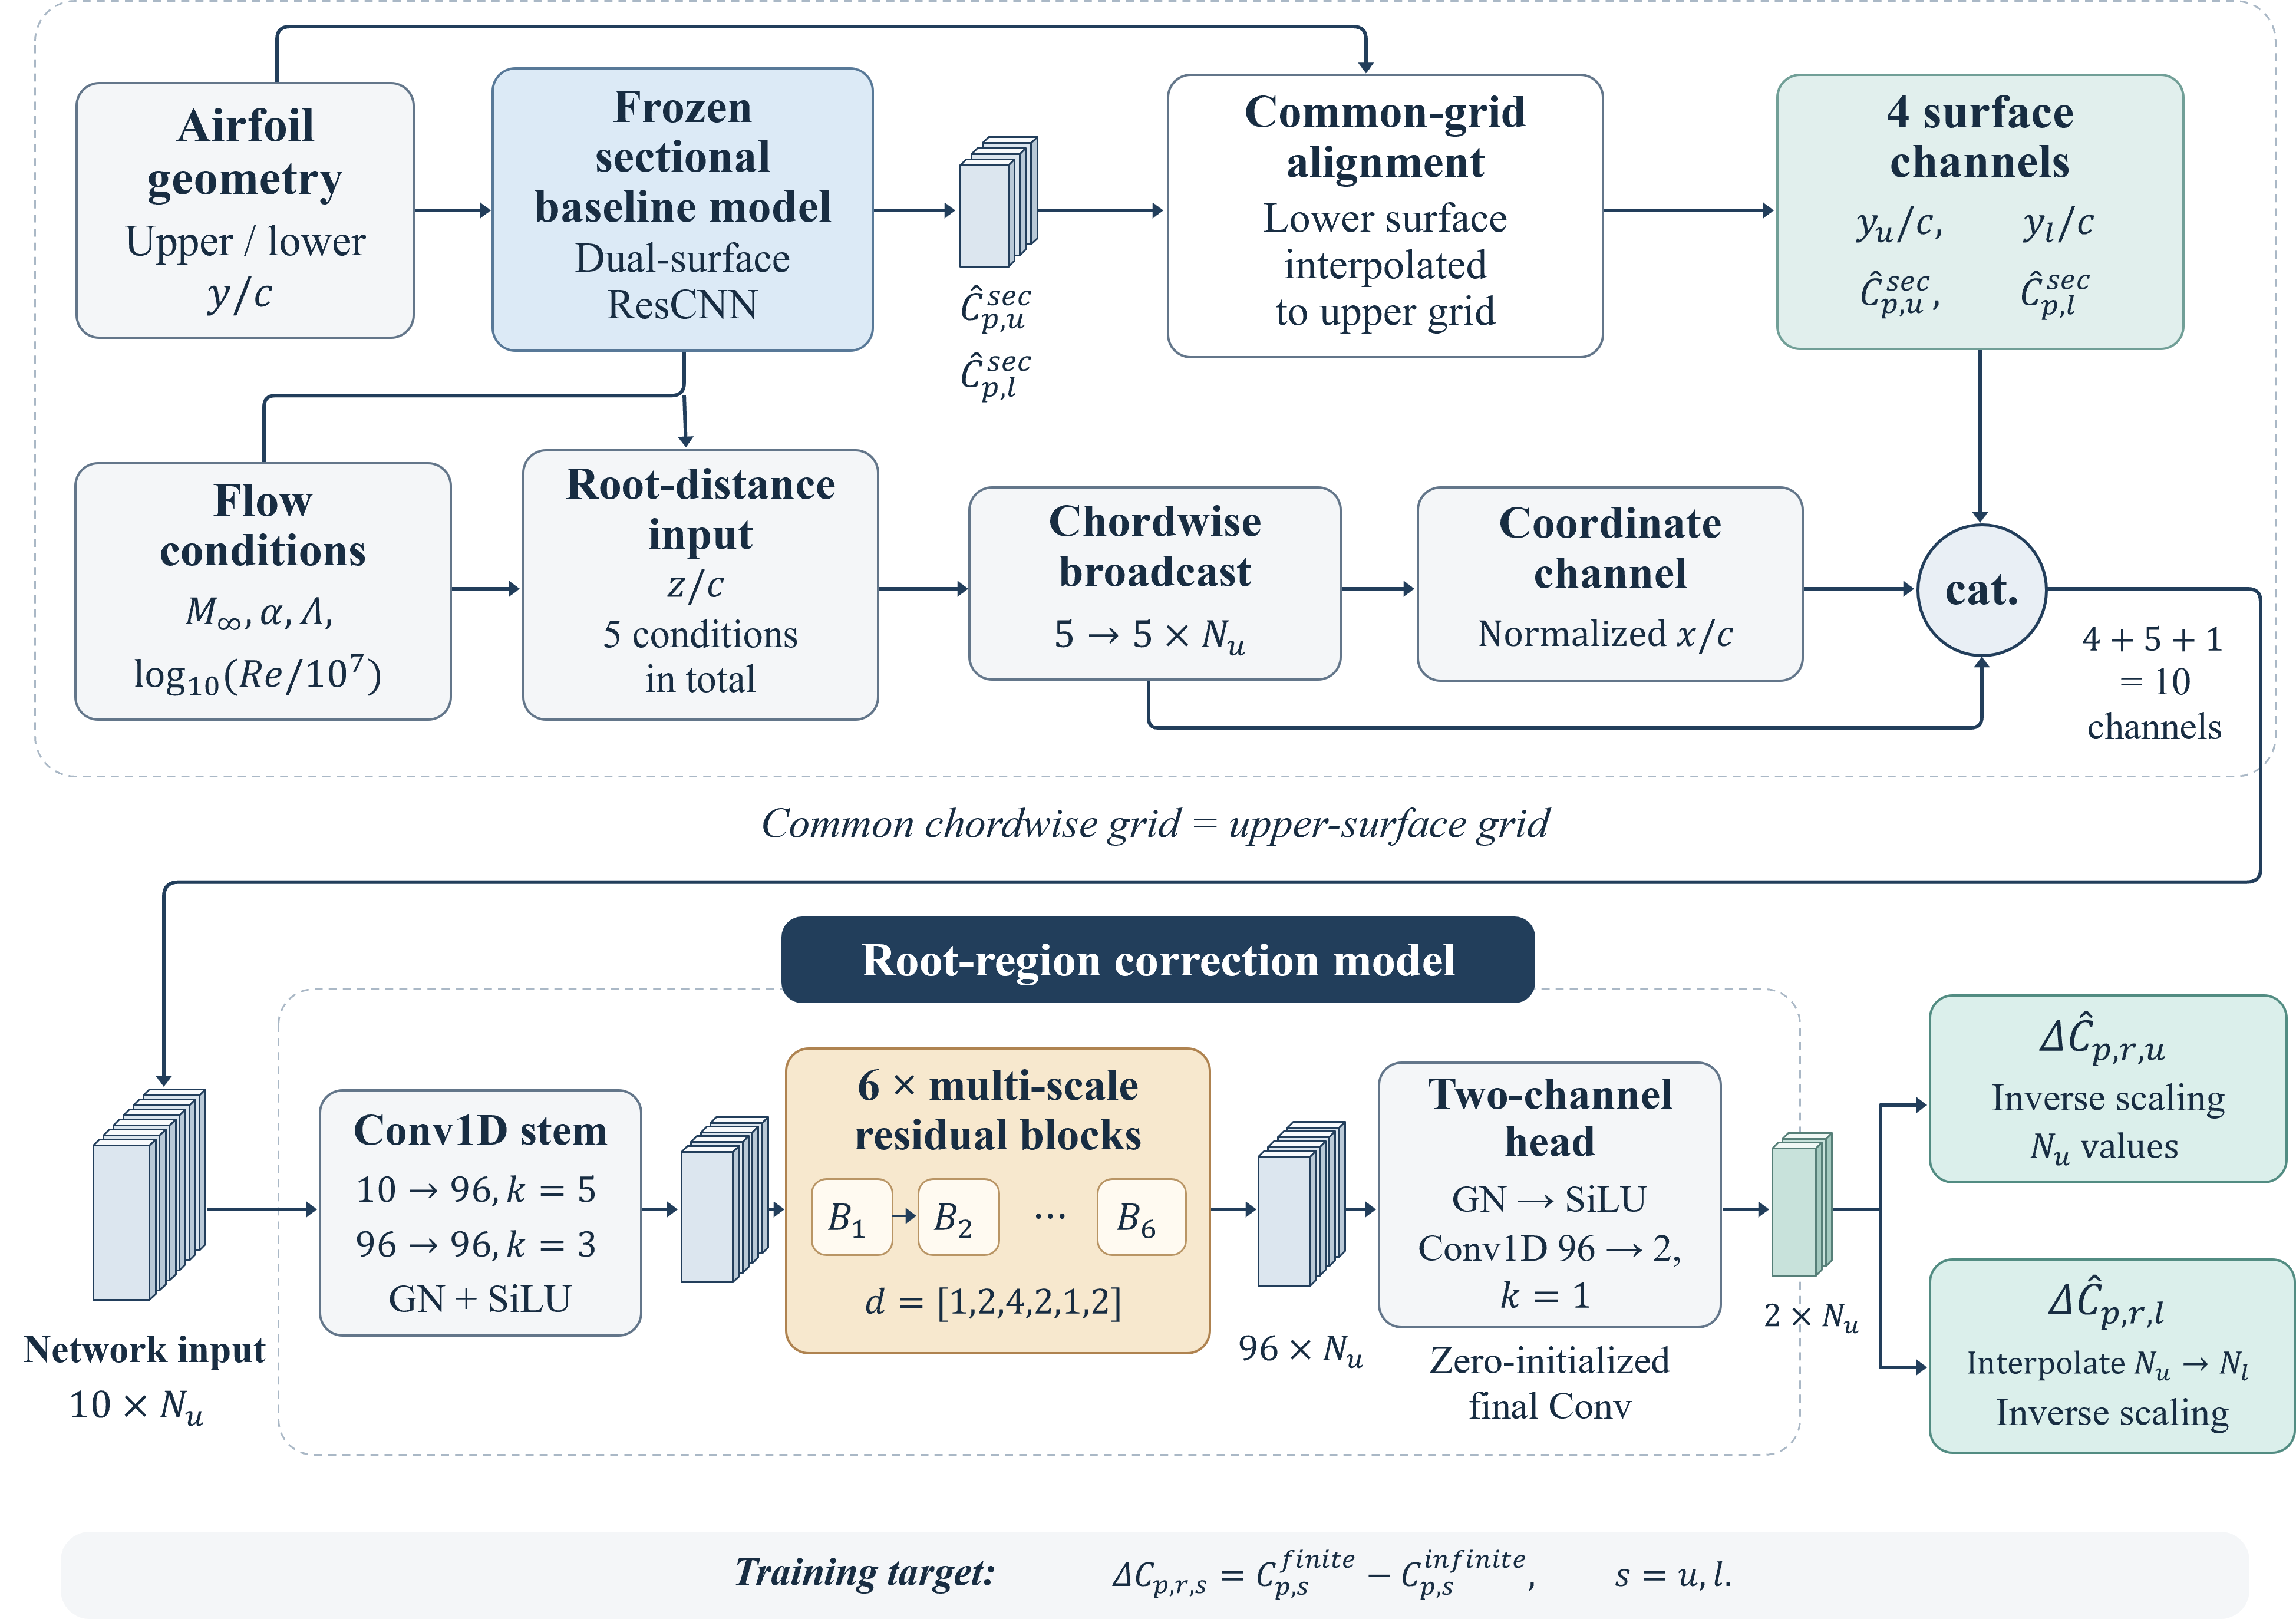
\includegraphics[width=\textwidth]{III_Knowledge_Transfer/figures/III_B_Fig10/III_B_Fig10_regional_architecture.png}
    \caption{Architecture of the root-region pressure-correction model conditioned on pretrained sectional predictions.}
    \label{fig:regional-architecture}
\end{figure*}
